\section{Implementation Diagnostics}

The numerical work in this paper checks the implementation of the theorem components on synthetic data only. These checks do not prove the theorem; they are regression-style diagnostics for whether the implemented finite-volume formulas satisfy the same conservation, CFL, and positivity quantities used in the proof.

The reported diagnostic run used a \(48\times40\) periodic grid on \([0,1]\times[0,1]\), a smooth positive depth field, smooth periodic velocity perturbations, nonnegative suspended sediment, and initial \(\beta=0\). The final time was \(T=0.05\). At every candidate step, the code checked both the hydrodynamic CFL condition and the local outgoing-flux sediment CFL. If either bound failed, the step size was reduced and the step was recomputed from the previous accepted state.

\begin{table}[H]
\centering
\caption{Summary of theorem-component diagnostics}
\begin{tabular}{lr}
\toprule
Quantity & Value \\
\midrule
Accepted steps & \(32\) \\
Final time & \(0.05\) \\
Maximum water-mass error & \(1.1102230246251565\times 10^{-16}\) \\
Maximum total sediment-volume error & \(0.0\) \\
Minimum depth & \(0.9207608559443589\) \\
Minimum ratio \(m^{n+1}/m^n\) & \(1.000373183439133\) \\
Minimum advected sediment \(s^*\) & \(0.030045021067309604\) \\
Minimum post-deposition sediment \(s\) & \(0.030042756519181715\) \\
Minimum concentration \(c=s/h\) & \(0.030007313661758465\) \\
Maximum hydrodynamic CFL & \(0.47500000000000003\) \\
Maximum local sediment CFL & \(0.02963343875200863\) \\
Maximum global sufficient sediment CFL & \(0.08162726734897778\) \\
Total time-step reductions & \(31\) \\
\bottomrule
\end{tabular}
\end{table}

Figure \ref{fig:mass-errors} shows that the water mass and total suspended-plus-stored sediment volume remain at roundoff-level error in the diagnostic run. Figure \ref{fig:positivity} reports the tracked lower bounds for depth, advected sediment, post-deposition sediment, and concentration. Figure \ref{fig:cfl} shows that accepted time steps stay within the two CFL restrictions.

\begin{figure}[H]
\centering
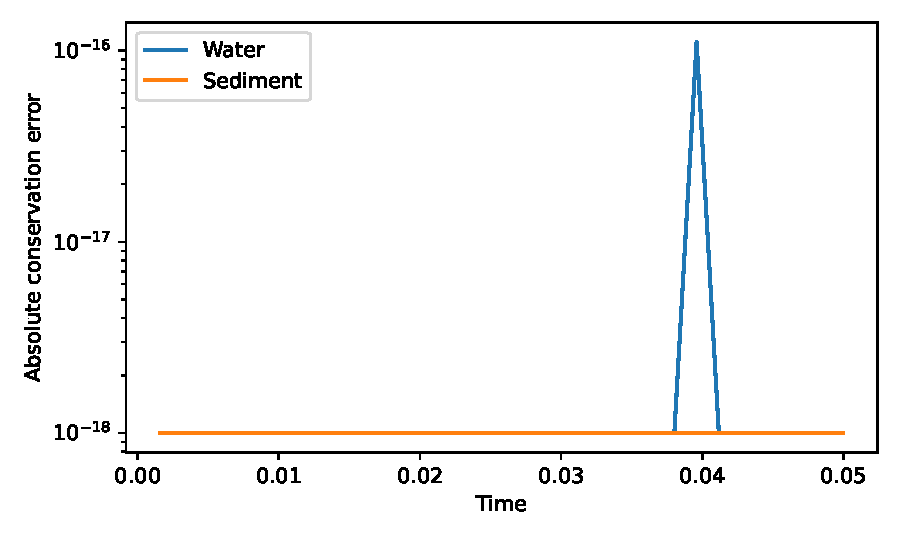
\includegraphics[width=0.82\textwidth]{figures/theorem_mass_errors.pdf}
\caption{Water-mass and sediment-volume accounting errors for the synthetic theorem diagnostic run.}
\label{fig:mass-errors}
\end{figure}

\begin{figure}[H]
\centering
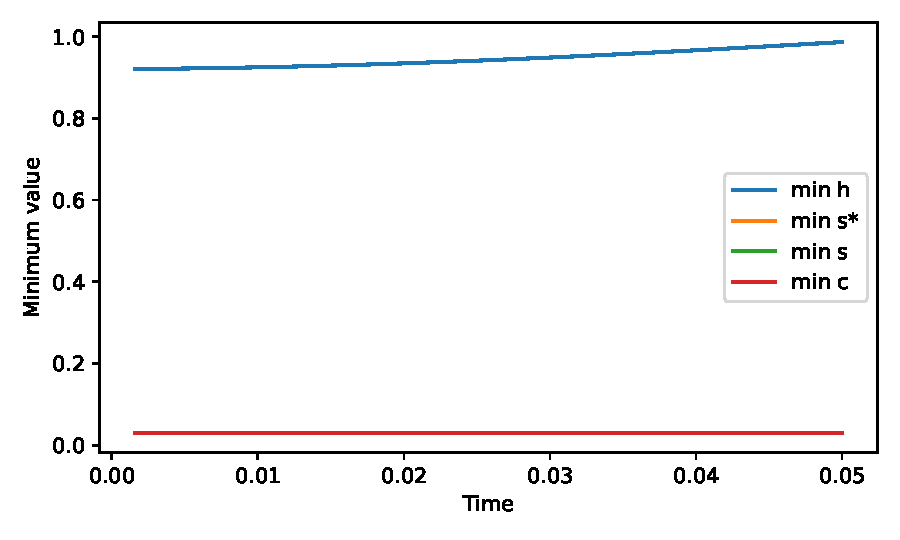
\includegraphics[width=0.82\textwidth]{figures/theorem_positivity_checks.pdf}
\caption{Tracked positivity diagnostics for depth, advected sediment, post-deposition sediment, and concentration.}
\label{fig:positivity}
\end{figure}

\begin{figure}[H]
\centering
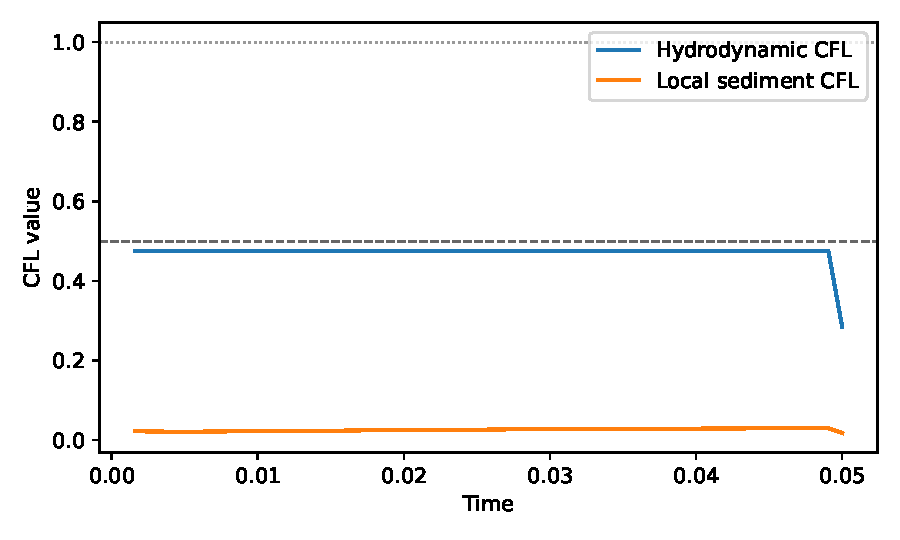
\includegraphics[width=0.82\textwidth]{figures/theorem_cfl_history.pdf}
\caption{Hydrodynamic and sediment CFL histories for accepted time steps.}
\label{fig:cfl}
\end{figure}

Additional synthetic checks were used for audit purposes: a constant periodic hydrodynamic state, a deposition-only test, a nonuniform periodic test, a near-CFL test, and a time-step retry test. The audit found that the code matches the approved finite-volume formulas and that the tests passed with tolerances of \(10^{-12}\) for mass, state, formula, positivity, and CFL diagnostics.
